\documentclass[a4paper,11pt,final]{article}

\usepackage[english,francais]{babel}
\usepackage[utf8]{inputenc}
\usepackage[T1]{fontenc}
\usepackage[pdftex]{graphicx}
\usepackage{setspace}
\usepackage{hyperref}
\usepackage[french]{varioref}
\usepackage{graphicx}
\usepackage{textcomp}
\usepackage[absolute]{textpos}
\usepackage{datetime}

\newcommand{\reporttitle}{Inversion de couleurs} 
\newcommand{\reportauthor}{Valentin \textsc{Durand}} 
\newcommand{\reportsubject}{TPE : Fondements de l'informatique} 
\newcommand{\HRule}{\rule{\linewidth}{0.5mm}}
\setlength{\parskip}{1ex} 
\setlength{\textwidth}{150mm}
\setlength{\oddsidemargin}{5mm}
\setlength{\topmargin}{0mm}
\setlength{\textheight}{220mm}
\newdate{date}{20}{01}{2017}
\date{\displaydate{date}}

\hypersetup{
    pdftitle={\reporttitle},%
    pdfauthor={\reportauthor},%
    pdfsubject={\reportsubject}
}

%% Le titre du papier
\title{Systèmes Temps Réel : \textsc{Projet}}
\author{Valentin Durand \texttt{<vdurand@ecole.ensicaen.fr>}\\Antoine Provot \texttt{<provot@ecole.ensicaen.fr>}}

\begin{document}

\begin{textblock*}{3cm}(85mm,20mm) 
	
\includegraphics[scale=0.2]{./pic/logo-ensicaen-2015.jpg} 
\end{textblock*} 

\maketitle

\section*{Travail préparatoire}
\begin{enumerate}
\item La tension évolue linéairement avec la température à raison de 10 mV/\textdegree C, sachant que la tension à 0\textdegree C est de 500 mV, si on mesure 850 mV alors la température sera d'environ 35\textdegree C.
\[T=\frac{U\cdot10^{-3}-500}{10}\]
\item Pour une tension de 850 mV, la valeur de l'adc sera 264.
\[ADC=\frac{U\cdot10^{-3}\times1024}{3300}\]
\item Architecture logiciel
\begin{figure}[!ht]
    \centering
    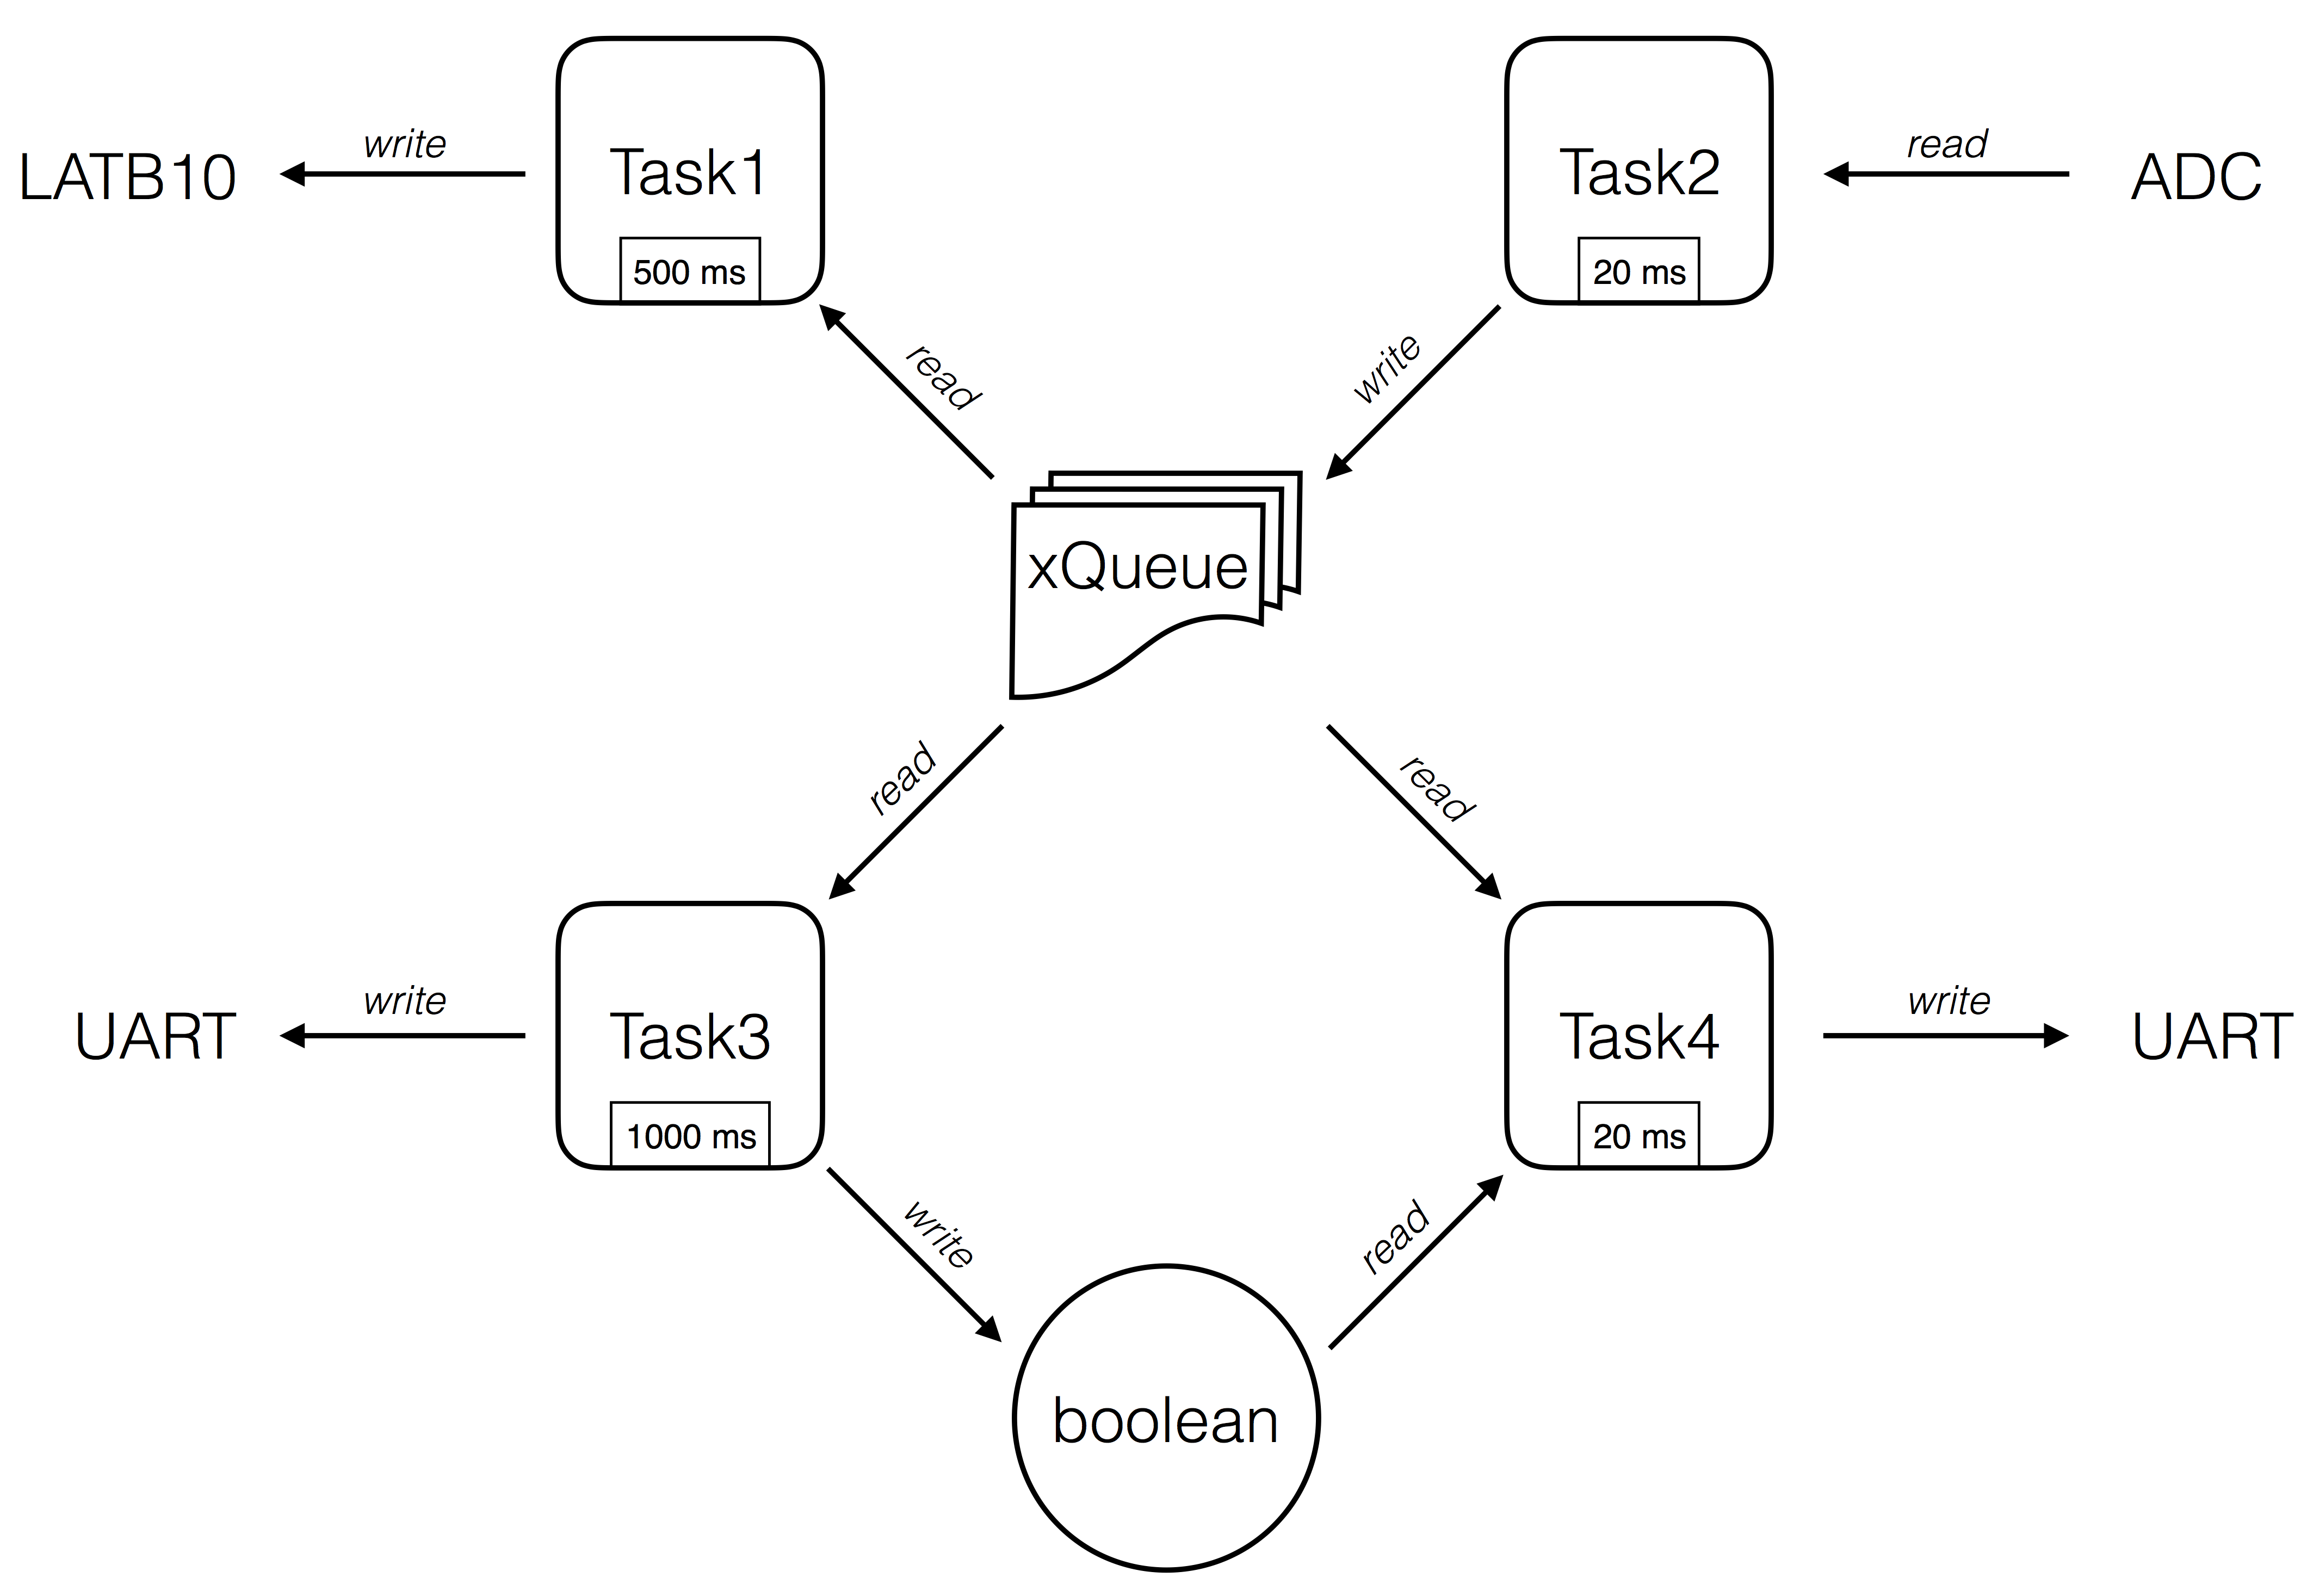
\includegraphics[width=130mm]{./pic/rtosdiag.png}
\end{figure}
\end{enumerate}

\section*{Description de l'architecture}

Notre projet comporte quatre tâches afin de gérer les fonctionnalités de l'application. Task2 de haute priorité, se charge de lire toutes les 20 ms la valeur de l'adc et de stocker la température dans une queue. 

Task1 s'occupe ensuite de lire les valeurs de la queue toute les 500 ms, si la valeur lue est inférieure à 38\textdegree C alors elle inverse la valeur de LATB10 pour provoquer un clignotement, si la valeur est supérieure elle met LATB10 à 1.

Task3 lit les commandes de l'utilisateur et provoque soit une lecture depuis la queue pour la commande read et dump, soit elle met un booléen à vrai pour activer l'affichage de la température dans la task4.

Task4 affiche donc la température lue depuis la queue avec une périodicité de 20 ms si le booléen est vrai, sinon elle ne fait rien.

\section*{Amélioration}

L'application pourrait être améliorée en utilisant une interruption pour faire clignoter la LED et en utilisant un sémaphore pour synchroniser les tâches 3 et 4.

\end{document}